\documentclass[11pt,a4paper]{article}
\usepackage[onecolumn,papersize=a4paper,margin=2.2cm,parskip]{kr-zh}

\usepackage{listings}
\usepackage{tabularx}
\usepackage{longtable}
\usepackage{subcaption}
\usepackage{xcolor}
\usepackage{graphicx}

\usepackage{float}
\usepackage{booktabs}
\usepackage{multirow}
\usepackage{graphicx}
\usepackage{caption}

\usepackage[backend=biber,style=numeric,natbib=true]{biblatex}
\addbibresource{references.bib}

\title{KELP: Closing the Knowledge–Exercise Loop for Learning Path Recommendation}

% Single author syntax
\author{%
    Zijie Liao
    \affiliations
    Guangdong Institute of Smart Education, Jinan University, Guangzhou, China
    \emails
    fenglin@stu2025.jnu.edu.cn
}


\begin{document}
\maketitle

\begin{abstract}
随着在线教育平台的广泛应用，如何为大规模学习者提供符合其个体需求的有效学习指导已成为自适应学习的重要问题。学习路径推荐旨在根据学习者状态与学习目标动态规划个性化学习序列。现有方法通常在知识点层面进行粗粒度规划，难以刻画不同习题的差异化作用；部分习题级方法虽然细化了推荐对象，但知识点规划与习题选择之间仍缺乏及时、有效的协同，导致路径规划不够灵活且局部学习效率受限。为此，本文提出细粒度学习路径推荐框架KELP，通过逐题反馈连接知识点规划与习题执行。KELP通过利用混合过程奖励缓解了强化学习模型奖励稀疏的问题,从而增强知识点规划能力，使系统能够根据持续变化的学习状态灵活调整路径；同时，通过面向当前目标知识点的局部执行机制选择高收益习题，使习题选择与当前知识点规划目标保持一致。通过闭合的知识点和习题循环实现了知识点路径的灵活规划和知识点的高效学习,从而提高了学生的学习有效性.我们在三个公开数据集上进行了大量的实验，KELP框架均取得了更优的学习收益，验证了所提出框架的有效性。
\end{abstract}

\section{Introduction}
随着在线教育平台的快速发展，学习者可以自由访问海量学习资源\cite{korableva2019studying,zhang2019hierarchical}。然而，面对内容、难度和知识关联各异的学习材料，学习者往往难以自主确定合适的学习顺序。学习路径推荐（Learning Path Recommendation, LPR）旨在根据学习者状态与学习目标生成个性化学习项目序列，从而提高目标导向学习的有效性\cite{nabizadeh2020learning,guan2025explainable,liu2019exploiting}。

早期LPR方法主要依赖规则、知识结构、优化算法或序列推荐技术，根据先修关系、相似学习者或历史行为模式生成路径\cite{nabizadeh2020learning,cover1967nearest,hidasi2015session}。这类方法具有一定可解释性或行为建模能力，但通常并不直接优化学习收益。随着知识追踪技术能够估计学生状态，强化学习逐渐成为LPR的重要范式。按推荐对象粒度，强化学习式LPR可分为知识点级与习题级两类：知识点级方法将学习抽象为概念序列，如CSEAL利用认知导航约束选择\cite{liu2019exploiting}，GEHRL规划多目标知识点顺序\cite{li2023graph}，SRC和LIGHT从目标集合生成完整路径\cite{chen2023set,yu2025light}，UNO利用过程奖励优化逐步知识点推荐\cite{peng2026uno}；习题级方法则进一步面向真实作答项目，如DLPR引入习题难度,将知识点的学习建模为独立的规划问题\cite{zhang2024item}，KnowLP基于知识结构与难度匹配选择习题\cite{cheng2026graphrag}，GenAL和ReAL结合题目文本、语义或相似学习者经验进行逐题推荐\cite{lv2025genal,lv2025real}。

尽管上述方法取得了进展，现有细粒度LPR仍存在三个关键问题。首先，奖励机制对于强化学习式LPR的训练效果有很重要的影响。UNO指出，以往方法主要使用终局奖励，只有在完整学习路径结束后才能获得反馈，因而面临典型的奖励稀疏问题；为此，UNO提出过程级的离散达成收益，即根据相邻时刻目标集合中达到掌握阈值的知识点数量变化来计算奖励。然而，这一改进仍不足以完全缓解奖励稀疏：当学生对目标知识点已有提升但尚未跨越阈值，或已达阈值后继续巩固时，离散达成收益仍可能为零，难以区分这些有效学习步骤。其次，现有规划策略的灵活性仍不足：知识图谱约束、固定子目标或阶段练习上限可降低复杂度，却也可能限制知识点切换、回访和练习次数调整；同时，现有方法难以根据学生当前的掌握情况灵活调整整体策略。最后，输出具体习题并不必然带来高效学习，难度匹配或文本/相似学习者驱动的选题未直接优化当前知识点目标收益,而将知识点的学习构建为独立的规划问题忽略了习题对于其他知识点的影响.

我们认为，有效的细粒度LPR应同时具备三点能力。第一，细粒度奖励机制应在离散达成收益之外引入连续掌握收益，即利用目标集合整体掌握度变化刻画每一步学习带来的连续状态变化，使策略能够在较大动作空间中获得更明确的判断信号，而不必过度依赖固定认知导航或A*\cite{duchovn2014path}式路径搜索。第二，知识点规划应具有逐题调整能力，并区分目标尚未达成时的推进需求与目标达成后的巩固需求。第三，当学生处于某一状态并需要提升某个知识点时，系统应像有经验的教师一样，从相关习题中选择对当前目标更有帮助的练习。如图~\ref{fig:method-comparison} 所示，细粒度LPR的关键不只是把推荐对象下沉到习题，还要闭合知识点规划与习题执行之间的反馈循环。
\begin{figure} % 位置参数，见下文解释
    \centering % 图片居中
    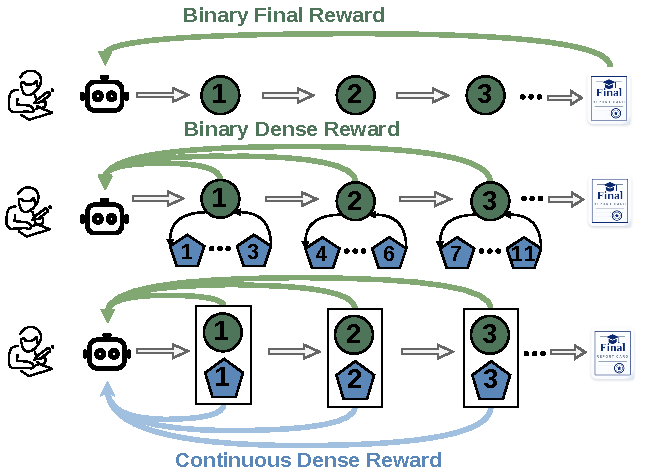
\includegraphics[width=\columnwidth]{illustration_new.pdf} % 插入图片并设置宽度
    \caption{Motivating comparison of reward design and decision granularity for fine-grained learning path recommendation.}
    \label{fig:method-comparison} % 用于交叉引用的标签
\end{figure}

为此，本文提出知识点--习题循环规划（Knowledge-Exercise Loop Planning, KELP），将基于混合奖励的知识点规划与监督式局部习题执行统一到逐题交互闭环中。具体而言，KELP首先利用离散达成收益与连续掌握收益构建混合过程奖励，使L-Agent能够自动学习下一步需要提升的知识点；其次，KELP将学习过程划分为目标推进与目标巩固两个阶段，以适应学生在不同目标完成状态下的决策需求；最后，KELP设计了基于状态感知双塔结构的bandit式局部执行器，通过候选扩展和一步前瞻收益监督学习高效习题选择策略。在三个公开数据集上的大量实验验证了本文方法的有效性，主要贡献总结如下：
\begin{itemize}
\item 提出离散--连续混合过程奖励，在保持目标达成导向的同时提供连续掌握收益，从而缓解阈值式过程奖励仍可能产生的稀疏反馈问题。
\item 提出逐题反馈驱动的两阶段知识点规划机制，使规划器能够在每次交互后自主继续、切换或回访知识点，并结合剩余预算适应目标推进与巩固阶段的不同需求。
\item 提出监督式局部习题执行器，通过图辅助候选扩展、状态感知双塔匹配和一步前瞻收益监督，提高面向当前知识点目标的习题选择质量。
\end{itemize}
\section{Related Work}
\subsection{学习路径推荐}
学习路径推荐旨在根据学习者的知识状态与学习目标，个性化地规划有序的学习项目序列\cite{nabizadeh2020learning}。早期方法采用协同过滤、KNN、GRU4Rec等序列推荐技术\cite{cover1967nearest,hidasi2015session}，但以重构行为序列为目标，未直接优化学习效果。近年来，知识追踪（Knowledge Tracing, KT）技术\cite{piech2015deep,shen2022assessing,liu2025deep}的发展使系统能够动态估计学生知识状态\cite{kubotani2021rltutor}.为此，研究者引入强化学习将LPR建模为序贯决策问题,按推荐对象粒度，学习路径推荐可分为知识点级与习题级方法。知识点级方法将学习过程建模为概念序列：CSEAL利用认知导航约束知识点选择\cite{liu2019exploiting}，GEHRL通过分层强化学习分解多目标规划\cite{li2023graph}，SRC和LIGHT生成完整知识点路径\cite{chen2023set,yu2025light}，UNO则利用KT过程奖励优化逐步知识点推荐\cite{peng2026uno}。此类方法降低了规划复杂度，但不区分同一知识点下的具体习题。

习题级方法进一步面向真实作答项目进行推荐。DLPR在分层规划中引入习题难度\cite{zhang2024item}，KnowLP基于知识结构与难度匹配选择习题\cite{cheng2026graphrag}，GenAL和ReAL利用大语言模型、题目语义或相似学习者经验辅助逐题推荐\cite{lv2025genal,lv2025real}。这些研究推动了细粒度推荐，但知识点规划与习题选择的协同仍有提升空间。本文进一步关注逐题反馈驱动的知识点规划与面向当前知识点目标的习题执行。
\subsection{强化学习}
强化学习通过智能体与环境持续交互，并依据累积奖励学习长期决策策略。奖励稀疏或延迟时，大量交互缺少可区分的监督，容易造成探索困难、时间信用分配困难与价值估计不稳定。现有研究主要从三个方向缓解这些问题：通过目标重标记从失败轨迹中构造额外监督\cite{andrychowicz2017hindsight}，通过分层策略与内部奖励将长时任务分解为较短子任务\cite{kulkarni2016hierarchical}，以及通过回报重分配将延迟收益归因至关键决策步骤\cite{arjona2019rudder}。在强化学习式LPR中，知识结构约束、分层子目标与过程奖励也可分别视为缩小探索空间、缩短信用分配时域和增强步级监督的具体实现\cite{liu2019exploiting,li2023graph,zhang2024item,peng2026uno}。

不同缓解机制作用于奖励稀疏问题的不同环节：结构先验与任务分解主要降低探索和信用分配难度，但并不直接增加每一步的奖励信息，其有效性也取决于预设结构与环境动态是否匹配。已有分层强化学习研究通过自主学习选项减少对预定义子目标的依赖，并指出任务特定层级设计及静态子目标机制在泛化和动态适应方面存在局限\cite{bacon2017optioncritic,nachum2018dataefficient,gurtler2021timed}。UNO设计的过程奖励虽然能够提供更及时的反馈，但当其基于阈值达成状态计算时，未跨越阈值的有效学习步骤仍可能获得零奖励。基于此，KELP在离散达成收益之外引入连续掌握收益，使学生状态的渐进改善也能够形成反馈，从奖励层面进一步缓解过程信号稀疏。


\section{Problem Formulation}
记知识点集合为 $\mathcal{K}$，习题集合为 $\mathcal{I}$，知识结构图为 $\mathcal{G}=(\mathcal{K},\mathcal{E})$。在时刻 $t$，知识点掌握状态记为 $h_t\in[0,1]^{|\mathcal{K}|}$，其中 $h_t(k)$ 表示学生对知识点 $k$ 的掌握程度；题目级作答概率状态记为 $p_t\in[0,1]^{|\mathcal{I}|}$，其中 $p_t(i)$ 表示学生正确回答习题 $i$ 的概率。由于真实学习日志主要记录题目级交互，本文依据知识追踪模型和题目--知识点映射，从同一历史序列中估计上述两类状态\cite{liu2025deep}。为衡量目标导向学习效果，定义时刻 $t$ 在目标集合上的离散目标达成量和连续掌握量为
\begin{equation}
\begin{aligned}
Q_t^N &= \sum_{k\in\hat{\mathcal{G}}}
\mathbb{I}\!\left(h_t(k)\geq\tau\right),\\
Q_t^S &= \sum_{k\in\hat{\mathcal{G}}} h_t(k),
\end{aligned}
\end{equation}
其中 $\tau$ 为掌握阈值，学习会话开始时目标集合尚未被完全掌握。时刻 $t$ 的归一化学习效果指标定义为
\begin{equation}
\begin{aligned}
E_t^N &= \frac{Q_t^N-Q_0^N}{|\hat{\mathcal{G}}|-Q_0^N},\\
E_t^S &= \frac{Q_t^S-Q_0^S}{|\hat{\mathcal{G}}|-Q_0^S}.
\end{aligned}
\end{equation}
最终评估指标分别记为 $E_N=E_T^N$ 和 $E_S=E_T^S$：前者衡量离散目标达成进度，后者衡量连续掌握进度；

本文关注目标导向的学习路径推荐问题。给定学习者历史 $\mathcal{H}$、目标集合 $\hat{\mathcal{G}}$ 与有限学习预算 $T$，系统需要逐步生成学习路径
$
\mathcal{P}=((g_1,e_1),\dots,(g_T,e_T)),
$
其中 $g_t\in\mathcal{K}$ 表示时刻 $t$ 选择的知识点，$e_t\in\mathcal{I}$ 表示围绕该知识点推荐的习题。时刻 $t$ 的剩余预算记为 $b_t=T-t+1$。本文的目标是在预算约束下学习知识点规划策略 $\pi^h_\theta$ 与监督式局部习题执行器 $f_\psi$，使生成路径在目标集合上最大化最终学习效果指标 $E_N$ 与 $E_S$。

\section{方法}
\subsection{总体框架}
\begin{figure*}[htbp]
  \centering
  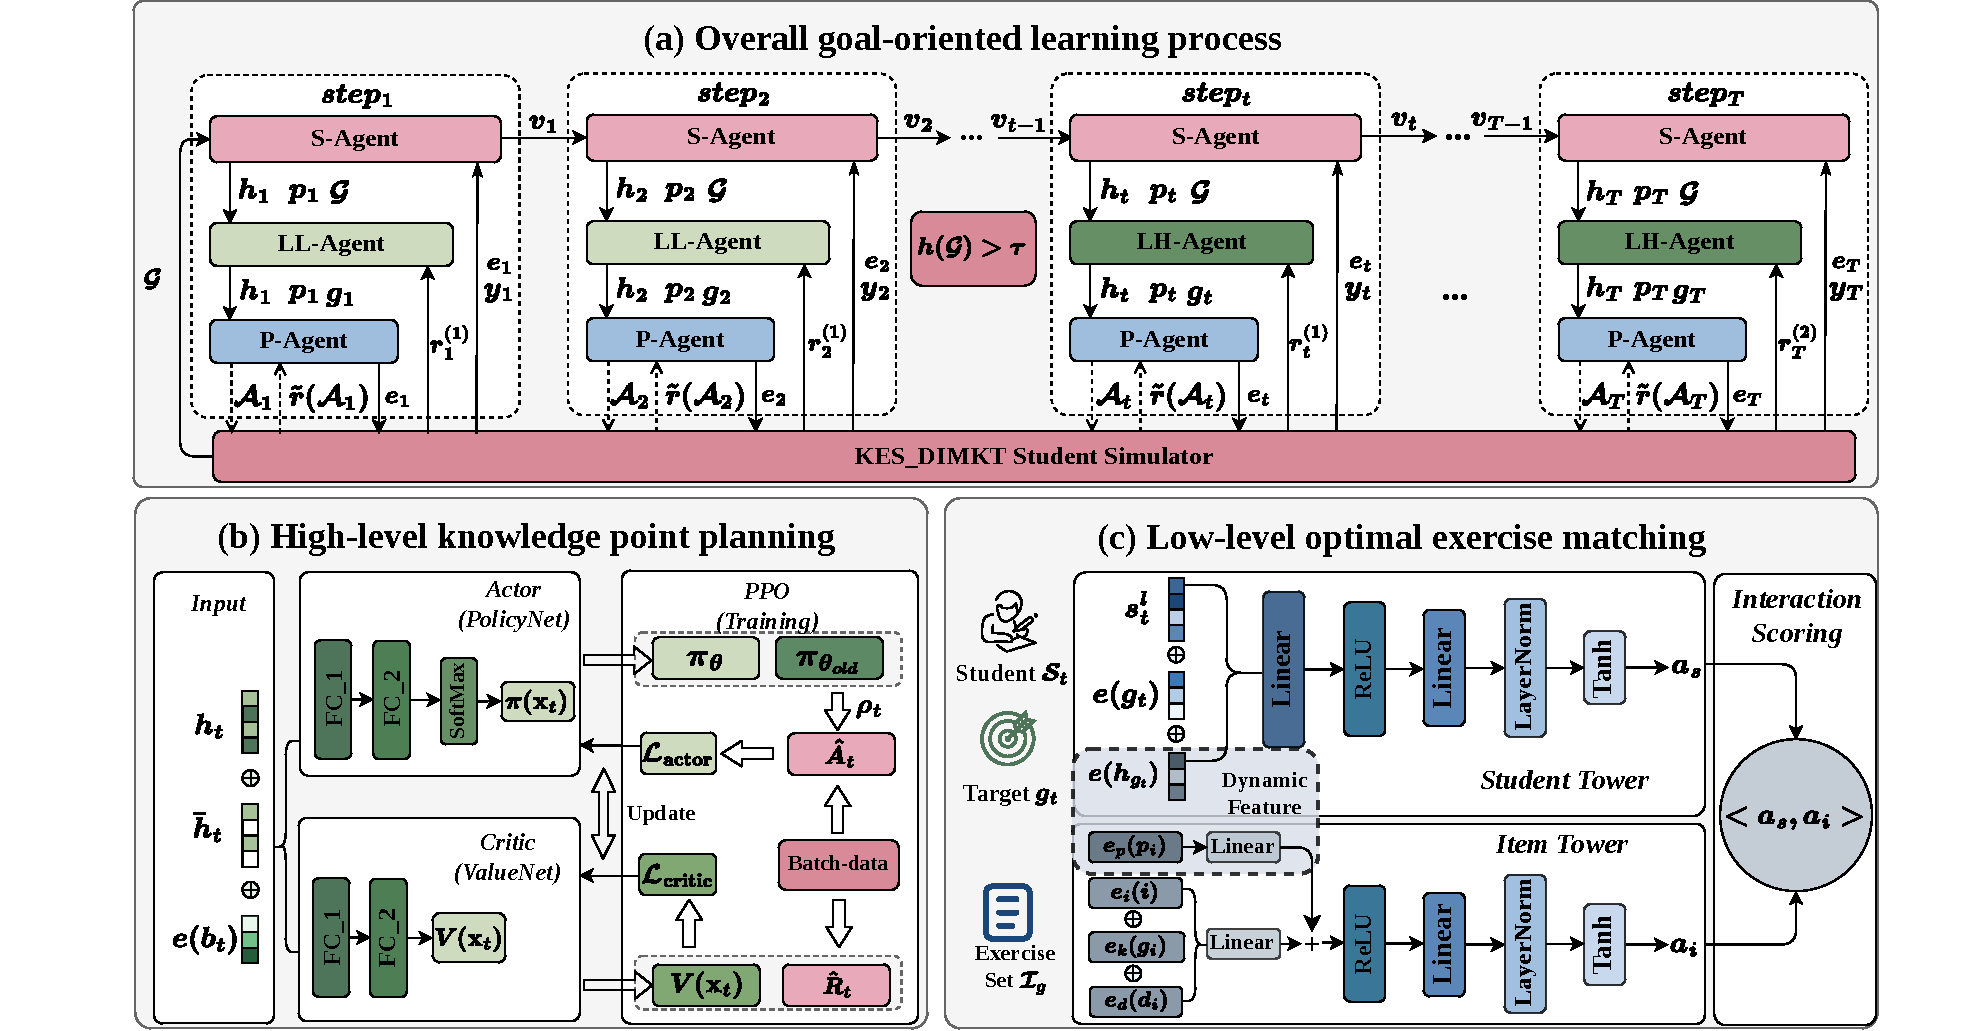
\includegraphics[width=1.0\textwidth]{framework.pdf} % 换成你的图
  \caption{\textbf{Framework overview of KELP.} (a) Exercise-synchronized goal-oriented learning process. (b) Knowledge point planning with discrete-continuous hybrid process rewards. (c) Supervised local exercise execution using graph-assisted candidate expansion and state-aware two-tower matching.}
  \label{fig:framework}
\end{figure*}
如图~\ref{fig:framework} 所示，KELP由学生状态估计模块 S-Agent、知识点规划器 L-Agent、监督式局部习题执行器与学生模拟器组成。图~\ref{fig:framework}(a)展示整体闭环：在时刻 $t$，S-Agent根据历史交互估计状态 $(h_t,p_t)$；L-Agent结合目标集合与剩余预算选择知识点 $g_t$；局部执行器围绕该知识点选择习题 $e_t$；学生完成练习后，模拟器返回作答反馈 $y_t$ 并产生下一时刻状态。该闭环以一道习题为完整决策周期，因此L-Agent在每次交互后均可重新规划知识点。

图~\ref{fig:framework}(b)展示知识点规划。L-Agent是框架中使用强化学习的规划模块，其利用离散--连续混合过程奖励学习知识点策略，并根据目标完成情况分别执行目标推进与目标巩固。图~\ref{fig:framework}(c)展示监督式局部习题执行：执行器不参与知识点规划，而是利用知识图谱扩展与当前目标相关的习题候选，并通过状态感知的两塔模型选择最有助于提升该知识点的习题。

S-Agent与学生模拟器均采用预训练DIMKT模型，但二者参数相互独立。S-Agent用于根据可观测历史估计决策状态，学生模拟器则用于刻画环境中的状态转移，从而避免决策侧直接访问模拟器的内部状态\cite{liu2019exploiting}。

\subsection{习题同步的知识点规划}

\subsubsection{逐题重规划与知识点状态}

传统分层方法通常在阶段或子会话开始时确定高层目标，并在多次低层交互期间保持该目标不变。KELP仍保留“知识点规划--习题执行”的职责分解，但不为高层目标预先分配固定练习窗口。每完成一道习题，更新后的学生状态都会立即返回L-Agent，由其重新选择下一步知识点：
\begin{equation}
(h_t,p_t,b_t)
\xrightarrow{\pi^h_\theta}
g_t
\xrightarrow{f_\psi}
e_t
\xrightarrow{\mathrm{Sim}}
(h_{t+1},p_{t+1},b_{t+1}).
\end{equation}
因此，当 $g_{t+1}=g_t$ 时，系统继续练习当前知识点；当 $g_{t+1}\neq g_t$ 时，系统切换学习知识点；当 $g_{t+1}$ 等于更早时刻学习过的知识点时，系统实现知识点回访。三种行为均由同一高层策略根据最新状态自主决定。

结合图~\ref{fig:framework}(b)，L-Agent的状态由学生当前知识点掌握状态 $h_t$、目标感知状态 $\bar{h}_t=h_t\odot y$ 与预算嵌入 $e_b(b_t)$ 构成。其中，$y\in\{0,1\}^{|\mathcal{K}|}$ 为目标指示向量，当 $k\in\mathcal{G}_{target}$ 时有 $y(k)=1$，否则为 $0$。高层状态定义为
\begin{equation}
s_t^h=[h_t;\,\bar{h}_t;\,e_b(b_t)],
\end{equation}
其中，$h_t$描述学生的全局知识背景，$\bar{h}_t$突出目标集合上的实时进展，$e_b(b_t)$则使策略能够区分不同剩余学习预算下的决策需求。

\subsubsection{预算感知的双阶段策略}

目标导向学习包含目标推进与目标巩固两种不同需求：目标尚未完成时，应优先推动知识点达到掌握阈值；目标达成后，则可利用剩余预算维持并进一步提升掌握状态。单一策略难以同时兼顾两类目标，因此KELP维护两个独立的知识点策略。

当仍存在未达到掌握阈值 $\tau$ 的目标知识点时，系统激活LL-Agent执行目标推进；当全部目标知识点均达标且预算仍有剩余时，系统切换至LH-Agent进行目标巩固。对于阶段 $m\in\{1,2\}$，策略网络与价值网络根据高层状态 $s_t^h$ 分别输出知识点选择分布和长期回报估计：
\begin{equation}
\begin{aligned}
\pi_{\theta_m}^h( s_t^h)
&=
\mathrm{Softmax}\!\big(FC_{\theta_m}(s_t^h)\big),\\
\qquad
V_{\phi_m}(s_t^h)&=FC_{\phi_m}(s_t^h).
\end{aligned}
\end{equation}
两个阶段分别使用对应轨迹优化策略，但均保持习题同步的决策周期，即L-Agent在每道习题交互后重新规划知识点。

\subsection{离散--连续混合过程奖励}

\subsubsection{混合过程奖励与双阶段设计}

仅使用离散达成收益作为过程奖励时，奖励只有在目标知识点跨越掌握阈值后才会变化，因而无法反映未达阈值时的渐进改善以及达标后的进一步提升。为此，KELP联合使用一步离散达成收益与一步连续掌握收益，分别定义为
$
\Delta E_t^{N}=E_{t+1}^{N}-E_t^{N},
\Delta E_t^{S}=E_{t+1}^{S}-E_t^{S}.
$
其中，$\Delta E_t^{N}$为离散达成收益，用于判断当前交互是否推动目标知识点达标；$\Delta E_t^{S}$为连续掌握收益，用于判断当前交互是否产生了尚未体现为阈值跨越的有效学习进展。

在此基础上，为了使双阶段策略与其优化目标保持一致，我们分别构造目标推进与目标巩固阶段的过程奖励。阶段一的一步奖励写为
\begin{equation}
r_t^{h,1}
=
\Delta E_t^{N}
+
\Delta E_t^{S}
-
\eta
-
\xi_t,
\end{equation}
其中，$\eta$为固定步级惩罚，$\xi_t$表示预算耗尽但目标尚未完成时的终局惩罚，其幅度为 $\xi=\lambda_{\xi}(1-E_T^{N})$。混合过程奖励为策略提供逐步学习信号，步级惩罚与终局惩罚则促使策略在有限预算内提高目标推进效率。

当全部目标知识点均达到阈值且预算仍有剩余时，系统进入阶段二。此时，LH-Agent不再将“达标”作为主要优化方向，而是转而强调目标状态的稳定保持与进一步提升。阶段二奖励定义为:
\begin{equation}
r_t^{h,2}=2\Delta E_t^{S}-
\mu\,\mathbb{I}\!\left(\exists k\in\mathcal{G}_{target},\,h_{t+1}(k)<\tau\right)
-
\eta,
\end{equation}
其中，$\mu$为退化惩罚系数。阶段二主要利用连续掌握收益推动目标状态进一步提升；一旦某个目标知识点重新跌破阈值，退化惩罚将抑制可能破坏已达成目标的决策。

\subsubsection{L-Agent策略优化}

我们采用 PPO 对知识点策略进行优化.给定一条由知识点决策形成的交互轨迹，首先根据时序差分误差构造优势项：
\begin{equation}
\begin{aligned}
\delta_t &= r_t^{h,m}+\gamma V_{\phi_m}(s_{t+1}^h)-V_{\phi_m}(s_t^h),\\
\hat{A}_t &= \sum_{l=0}^{\infty}(\gamma\lambda)^l\delta_{t+l}.
\end{aligned}
\end{equation}
其中，$\gamma$表示折扣因子,$\lambda\in[0,1]$ 为 广义优势估计(GAE)中的衰减系数，用于调节优势估计在偏差与方差之间的权衡；较大的 $\lambda$ 使估计更多吸收长时域回报信息，而较小的 $\lambda$ 则使其更接近局部时序差分更新。随后，策略网络通过 PPO 裁剪目标进行更新：
\begin{equation}
\mathcal{L}_{actor}^{(m)}
=
-\mathbb{E}_t
\left[
\min\left(
\rho_t\hat{A}_t,\,
\mathrm{clip}(\rho_t,1-\epsilon,1+\epsilon)\hat{A}_t
\right)
\right],
\end{equation}
其中 $\rho_t=\pi_{\theta_m}^h(g_t\mid s_t^h)/\pi_{\theta_m^{old}}^h(g_t\mid s_t^h)$。价值网络基于冻结的价值估计构造 TD($\lambda$) 式目标回报，并通过平方误差进行更新：
\begin{equation}
\begin{aligned}
\hat{R}_t^{(m)}
&=\hat{A}_t+\hat{V}_{\phi_m}(s_t^h),\\
\mathcal{L}_{critic}^{(m)}
&=\mathbb{E}_t\!\left[
\left(V_{\phi_m}(s_t^h)-\hat{R}_t^{(m)}\right)^2
\right].
\end{aligned}
\end{equation}
其中 $\hat{V}_{\phi_m}(s_t^h)$ 表示在当前更新轮次开始时计算得到的价值基线。由于两个阶段分别维护独立的L-Agent，阶段一与阶段二的轨迹用于更新对应策略，使其分别学习目标推进和目标巩固偏好。

\subsection{图辅助的监督式局部习题执行}
L-Agent利用强化学习决定下一步需要提升的知识点，监督式局部习题执行器 $f_\psi$ 则负责完成该知识点目标。本文采用图~\ref{fig:framework}(c)所示的两塔结构学习学生与习题之间的匹配函数，并使用一步前瞻收益监督该局部选题过程。

\subsubsection{双塔匹配建模}

学生塔用于在当前学习知识点条件下生成学生侧状态表示。其输入由三部分组成：学生基础表征 $s_t^l=[p_t;\,h_t]$，其中 $p_t$ 和 $h_t$ 分别表示题目级与知识点级掌握状态；当前学习知识点的语义条件 $e_k(g_t)$；以及学生对该知识点的动态掌握特征 $e_h(h_t(g_t))$，用于突出当前局部学习需求。三类信息共同输入学生侧编码器，得到:
\begin{equation}
a_t^{u}
=
f_u\!\left([s_t^l;\,e_k(g_t);\,
e_h(h_{g_t})]\right),
\end{equation}
其中，$f_u(\cdot)$ 对应于图~\ref{fig:framework}(c)中的学生塔前馈编码网络。$a_t^u$ 表示知识点条件化的学生侧表示。

与之对应，习题塔同时整合习题静态特征与学生-习题交互相关的动态特征。对于任意候选习题 $i$，我们将题目标识嵌入$e_i(i)$、所属知识点嵌入$e_k(k_i)$与题目难度嵌入$e_d(d_i)$视为其静态描述.在此基础上，再引入题目级掌握度嵌入 $e_p(p_t(i))$ 作为动态补充,进而得到习题表示:
\begin{equation}
a_i^{v}
=
f_v\!\left(
W_s[e_i(i);\,
e_k(k(i));\,
e_d(d_i)]
+
W_p e_p(p_i)
\right),
\end{equation}
其中$W_s$ 与 $W_p$ 分别表示静态特征映射与动态特征映射，$f_v(\cdot)$ 为习题侧输出网络,$a_i^v$ 表示动态化的习题侧表示

在此基础上，我们采用内积形式衡量学生表示与习题表示之间的匹配强度，并将其作为当前状态下的习题适配得分输出：
\begin{equation}
\hat{r}_{t}(i\mid c_t^l,g_t)=\langle a_t^{u},a_i^{v}\rangle.
\end{equation}
该得分并不直接等价于作答正确概率，而是刻画题目 $i$ 在当前学习知识点 $g_t$ 及当前学生状态下的练习适配性。分数越高，表示该题越可能在当前局部学习阶段发挥有效练习作用。
\subsubsection{候选生成}

围绕当前知识点 $g_t$，我们首先依据知识点到习题的映射关系 $\mathcal{M}(k)$ 收集相关题目。同时，考虑到提升 $g_t$ 的最有效习题可能来自关联知识点，我们进一步为其根据其关联知识点的掌握状态自适应地引入一对邻近知识点：记
\begin{equation}
\begin{aligned}
\tilde{k}_t^{-}
&=
\arg\min_{k\in \mathrm{Pre}(g_t)} h_t(k),\\\qquad
\tilde{k}_t^{+}
&=
\arg\max_{k\in \mathrm{Suc}(g_t)} h_t(k),  
\end{aligned}
\end{equation}
其中 $\mathrm{Pre}(g_t)$ 与 $\mathrm{Suc}(g_t)$ 分别表示 $g_t$ 在知识图中的前置知识点集合与后继知识点集合。前者用于定位当前最薄弱的先修支撑点，后者用于定位当前掌握程度较高的后继关联点。于是，合法候选集合定义为
\begin{equation}
\mathcal{I}_t(g_t)
=
\mathcal{M}(g_t)\cup
\mathcal{M}(\tilde{k}_t^{-})\cup
\mathcal{M}(\tilde{k}_t^{+})
,
\end{equation}
当某一邻域集合为空时，对应项自然省略。在得到合法候选集合后，我们再由两塔网络在该集合上输出习题适配得分，并形成一个用于后续训练决策的小规模候选子集
\begin{equation}
\mathcal{A}_t
=
\mathrm{TopK}\!\left(\hat{r}_{t}(\cdot\mid c_t^l,g_t),K\right)
\cup
\mathrm{Rand}\!\left(\mathcal{I}_t(g_t),K_r\right).
\end{equation}
其中，$K$ 表示由两塔匹配得分筛出的高分候选数，$K_r$ 表示为保持候选多样性而额外加入的随机候选数。

\subsubsection{题目选择与监督学习}

在训练阶段，局部执行器并不直接把两塔打分最高的题目作为最终执行题目，而是对候选题进行一步前瞻评估。具体地，对于每个候选习题 $i\in\mathcal{A}_t$，记其对应的一步前瞻知识状态为 $\hat{h}_{t+1}^{(i)}$，并令
\begin{equation}
\tilde{r}_t(i)=
\hat{h}_{t+1}^{(i)}(g_t)-h_t(g_t),
\end{equation}
我们会选择收益最大的习题训练阶段真实执行的习题.同时该收益也作为训练时的监督信号，使局部执行器学习当前状态下更可靠的习题匹配函数。

在监督学习时，我们会保留同一候选集合 $\mathcal{A}_t$ 中各题目的 $(s_t^l,g_t,i,\tilde{r}_t(i))$。这样，模型能够同时观察“最终被选中的题目”与“在同一状态下未被选中的备选题目”，从而学习更稳定的局部偏序关系。记 $\bar{r}_t(i)$ 为对 $\tilde{r}_t(i)$ 进行组内标准化后得到的监督信号，则局部习题执行器的训练目标写为
\begin{equation}
\begin{aligned}
\mathcal{L}_{grp}
&=
\frac{1}{|\mathcal{P}_t|}
\sum_{(i,j)\in\mathcal{P}_t}
\mathrm{softplus}\!\big(
\hat{r}_{t}(j)-\hat{r}_{t}(i)
\big),\\
\mathcal{L}_{reg}
&=
\mathrm{SmoothL1}\!\left(
\hat{r}_{t}(i\mid c_t^l,g_t),\bar{r}_t(i)
\right),\\
\mathcal{L}_{exec}
&=
\lambda_{grp} \mathcal{L}_{grp}
+
\lambda_{reg} \mathcal{L}_{reg},
\end{aligned}
\end{equation}
其中，$\mathcal{P}_t=\{(i,j)\mid \tilde{r}_t(i)>\tilde{r}_t(j)\}$ 表示由模拟收益诱导的候选偏序集合；$\lambda_{grp}$ 与 $\lambda_{reg}$ 分别控制组内排序约束与收益回归约束的强度。前者推动模型在同一候选组内学习“哪道题更优”，后者则使预测得分与收益监督保持数值一致。

在推理阶段，我们不再使用上述一步前瞻收益，而是直接依据局部执行器已经学得的两塔匹配函数，在合法候选集内完成选题.
由此，混合过程奖励为L-Agent提供逐步知识点规划依据，习题同步架构使其能够在每次交互后立即调整规划，而监督式局部执行器负责完成当前知识点目标，三者共同形成细粒度闭环。
\section{实验}
\subsection{Datasets}
我们的方法建立在3个公开数据集之上:Junyi,Assist09,Assist17的基础之上.和DLPR一样,我们使用了转移图构建了Assist09和Assist17的知识图谱;根据Junyi数据集提供的一个习题级的先决关系图构建了知识点级的知识图谱;以及使用相同的方案计算知识点和习题的难度.需要提到的是,我们借助pyKT的数据预处理方案对这三个数据集进行处理,按照16:4:5将其划分为训练集,验证集,测试集.表~\ref{tab:datasets}展示了所有数据集的统计详情.
\begin{table}[H]
\centering
\captionsetup{labelfont=bf,textfont=bf}
\caption{Statistics of the datasets.}
\label{tab:datasets}
\setlength{\tabcolsep}{4pt}
\footnotesize
\begin{tabular}{cccc}
\toprule
\textbf{Dataset} & \textbf{Junyi} & \textbf{Assist09} & \textbf{Assist17}  \\
\midrule
Concept & 39 & 123 & 102 \\
Item & 721 & 17737 & 3162 \\
Learner & 191874 & 3852 & 1708 \\
Interaction & 25,853,987 & 337,424 & 942,814 \\
Difficulty & 26.87 & 34.29 & 53.91 \\
\bottomrule
\end{tabular}
\end{table}
\begin{table*}[t]
\centering
\captionsetup{labelfont=bf,textfont=bf}
\caption{Performance comparison on Junyi, Assist09, and Assist17. The best and second-best results in each row are highlighted in bold and underlined, respectively.}
\label{tab:main_results}
\setlength{\tabcolsep}{3.2pt}
\renewcommand{\arraystretch}{1.0}
\scriptsize
\resizebox{\textwidth}{!}{
\begin{tabular}{cccccccccccc}
\toprule
\textbf{Dataset} & \textbf{Indicator} & \textbf{Step} & \textbf{AC} & \textbf{PPO} & \textbf{GRU4Rec} & \textbf{SRC} & \textbf{CSEAL} & \textbf{GEHRL} & \textbf{DLPR} & \textbf{UNO} & \textbf{KELP} \\
\midrule
\multirow[c]{6}{*}{Junyi} & \multirow[c]{3}{*}{En} & 5  & 0.2487 & 0.3574 & 0.0912 & 0.4647 & 0.2516 & 0.2038 & \underline{0.5364} & 0.2898 & \textbf{0.5873} \\
 &  & 10 & 0.3407 & 0.5199 & 0.1646 & \underline{0.6410} & 0.3440 & 0.3090 & 0.6350 & 0.4216 & \textbf{0.8326} \\
 &  & 20 & 0.5145 & 0.6697 & 0.2392 & \underline{0.9473} & 0.4327 & 0.4463 & 0.6976 & 0.5666 & \textbf{0.9692} \\
\cmidrule(lr){2-12}
 & \multirow[c]{3}{*}{Es} & 5  & 0.0721 & 0.1286 & 0.0612 & 0.2168 & 0.0514 & 0.0669 & \underline{0.2348} & 0.1181 & \textbf{0.2586} \\
 &  & 10 & 0.1161 & 0.2146 & 0.1749 & \underline{0.3159} & 0.0867 & 0.1042 & 0.2493 & 0.1840 & \textbf{0.4464} \\
 &  & 20 & 0.1836 & 0.3295 & 0.1241 & \underline{0.6205} & 0.1364 & 0.1614 & 0.2746 & 0.2689 & \textbf{0.6761} \\
\midrule
\multirow[c]{6}{*}{Assist09} & \multirow[c]{3}{*}{En} & 5  & 0.3428 & 0.3375 & 0.3293 & 0.3476 & 0.2516 & 0.2867 & 0.1802 & \underline{0.4602} & \textbf{0.6881} \\
 &  & 10 & 0.4079 & 0.4729 & 0.1533 & 0.4205 & 0.3440 & 0.3685 & 0.2175 & \underline{0.4917} & \textbf{0.7496} \\
 &  & 20 & 0.4207 & 0.6063 & 0.1241 & \underline{0.6883} & 0.4143 & 0.4287 & 0.2466 & 0.4947 & \textbf{0.9165} \\
\cmidrule(lr){2-12}
 & \multirow[c]{3}{*}{Es} & 5  & 0.1530 & 0.1892 & 0.1721 & 0.2042 & 0.1128 & 0.1515 & 0.0194 & \underline{0.2269} & \textbf{0.5296} \\
 &  & 10 & 0.1435 & 0.2426 & 0.0058 & \underline{0.2848} & 0.1152 & 0.1476 & -0.0057 & 0.1909 & \textbf{0.5851} \\
 &  & 20 & 0.1382 & 0.3276 & 0.0131 & \underline{0.4318} & 0.1140 & 0.1523 & -0.0197 & 0.1659 & \textbf{0.7397} \\
\midrule
\multirow[c]{6}{*}{Assist17} & \multirow[c]{3}{*}{En} & 5  & 0.2941 & \underline{0.3108} & -0.0468 & 0.1995 & 0.0837 & 0.0191 & 0.1059 & \textbf{0.3796} & 0.2886 \\
 &  & 10 & 0.3747 & 0.4147 & -0.0041 & 0.4047 & 0.1681 & 0.0302 & 0.1920 & \underline{0.4225} & \textbf{0.4711} \\
 &  & 20 & 0.4440 & 0.7071 & 0.0068 & \underline{0.7859} & 0.2967 & 0.0442 & 0.1387 & 0.4386 & \textbf{0.9169} \\
\cmidrule(lr){2-12}
 & \multirow[c]{3}{*}{Es} & 5  & \underline{0.2349} & 0.1861 & 0.0290 & 0.2110 & 0.0953 & 0.0313 & 0.0466 & \textbf{0.2845} & 0.1976 \\
 &  & 10 & 0.2803 & 0.2601 & 0.0655 & 0.2561 & 0.1255 & 0.0289 & 0.0800 & \underline{0.2859} & \textbf{0.3114} \\
 &  & 20 & 0.2665 & 0.3202 & 0.0947 & \underline{0.4350} & 0.1726 & 0.0329 & 0.1039 & 0.2871 & \textbf{0.5765} \\
\bottomrule
\end{tabular}
}
\end{table*}

\subsection{Compared Methods}

为了证明我们方法的优越性,我们与以下方法进行对比:
\begin{itemize}
\item AC:使用DIMKT对学生状态进行建模,在其基础上使用基于步级奖励方式训练的标准Actor-Critic算法作为推荐器\cite{sutton1999policy}.
\item PPO:使用DIMKT对学生状态进行建模,在其基础上使用基于步级奖励方式训练的PPO算法作为推荐器\cite{schulman2017proximal}.
\item GRU4Rec:GRU4Rec 是一种基于 GRU 的序列推荐模型，把用户历史交互看成时间序列，用循环神经网络去预测“下一个最可能交互的项目”\cite{hidasi2015session}。
\item SRC:SRC 是一种 set-to-sequence 的学习路径推荐方法：先把目标知识点集合输入到概念感知编码器中，建模知识点之间的关系并得到整体表示,然后再由解码器根据这个表示按顺序逐步生成学习路径\cite{chen2023set}.
\item CSEAL:CSEAL根据学习者状态并通过使用一种认知导航算法限制强化学习动作空间来指导Actor-Critic网络实现学习路径推荐\cite{liu2019exploiting}.
\item GEHRL:GEHRL使用分层强化学习方法,通过高层 PPO 代理规划多目标学习顺序、低层 Actor-Critic 代理实现单目标的学习\cite{li2023graph}.
\item DLPR:DLPR在分层强化学习的基础上,引入习题层面的考虑,将高层建模为基于PPO和A*算法的知识点学习规划,将低层建模为基于Actor-Critic的具体知识点的练习规划\cite{zhang2024item}.
\item UNO:UNO是一种基于序列编码的强化学习推荐方法，它首先对学生历史作答序列进行表示学习以构建当前状态，再结合知识追踪辅助监督与 GRPO 式策略优化实现下一知识点推荐\cite{peng2026uno}。
\end{itemize}

\subsection{Implementation Detail}
我们基于 PyTorch\cite{paszke2019pytorch}、Gym\cite{brockman2016openai}实现整个框架，并采用 pyKT提供的代码对 DIMKT 进行预训练。将基于训练集训练得到的 DIMKT 模型作为S-Agent的核心，以提供决策侧的学生状态估计；将基于训练集与测试集合并数据训练得到的另一套 DIMKT 模型作为学生的模拟器，以刻画环境侧更接近真实演化过程的状态转移。

在当前实现中，知识点规划层采用两个独立的 PPO 智能体分别对应目标推进阶段与目标巩固阶段。参考在线教育中常用的及格标准，我们将知识点掌握阈值设置为 0.6，并将单个学习会话的最大决策预算限制为 20 步。与前文奖励设计对应，步级惩罚系数和终局惩罚系数分别取 0.03 和 1.0。局部习题执行器采用监督式双塔匹配模型；在候选重排阶段，系统从合法候选集合中保留 6 道高分题，并额外补充 10 道随机候选题，以兼顾候选质量与局部探索。训练阶段，执行器使用一步前瞻收益监督候选题评分，并联合优化组内排序损失与回归损失；两类损失的权重分别设置为 0.1 和 1.0。对于知识点规划层的 PPO 代理，我们使用 Adam\cite{kingma2014adam} 优化 Actor 和 Critic 网络；对于监督式局部习题执行器，我们采用带有小权重衰减的 AdamW\cite{loshchilov2017decoupled} 优化双塔匹配模型，并减少对局部候选习题的过拟合。

\subsection{Experiment Result}
表~\ref{tab:main_results}显示了本文方法在三个数据集上的大多数设置下都取得了最优结果，说明所提出的分层两阶段细粒度决策框架能够稳定提升目标导向学习路径推荐的整体效果。尤其在 Junyi 和 Assist09 上，本文方法在不同步数与两类指标下均表现出显著优势；在 Assist17 上，仅在 $Step=5$ 的极短学习过程中略低于个别基线。我们认为，这并非短期失效，而是面向长期目标优化的阶段性取舍：为在有限预算内最大化最终学习收益，本文方法在前 5 步更倾向于为后续阶段积累更有利的知识状态，因此虽在
短期上略有让步，但在 $Step=10$ 与 $Step=20$ 时重新取得最优结果。

进一步观察基线方法可以发现，AC 与 PPO 虽然建模更简单，但在多数设置下整体优于 CSEAL 和 GEHRL，并在部分场景下接近甚至超过 UNO。这表明，合理的奖励机制对学习路径推荐性能具有关键作用：即使不引入复杂结构，只要奖励能够准确反映学习增益，系统依然能够学到较优策略。SRC 同样表现出较强竞争力，其重要原因在于编码器--解码器框架支持大批量并行训练，能够在更短时间内利用更多学生数据，具有明显的工程化优势；相比之下，其余强化学习方法大多依赖串行交互训练。即便如此，本文方法仍在绝大多数设置下超越 SRC，说明将连续掌握收益、双阶段知识点决策与面向局部增益的习题选择统一起来，能够进一步提升目标导向学习路径推荐的性能上限。


\subsection{Ablation Study}
在图~\ref{fig:Ablation study}中,为分析关键模块的作用，我们在主模型基础上设计四个消融变体：w/o Dynamic 去除习题层动态特征，w/o step 去除剩余步数特征及对应步级惩罚，w/o L2 移除阶段二知识点策略，w/o Adaptive 移除自适应候选机制。从结果上看，完整模型在大多数设置下均取得最优表现，说明上述设计均对性能提升有积极作用。其中，去除动态特征后性能明显下降，表明基于具体知识点和习题的状态感知的局部匹配对习题推荐至关重要；去除预算感知后，中长预算下表现普遍变差，说明剩余步数特征及步级惩罚有助于提升知识点层的规划效率；移除阶段二策略后，部分连续收益指标 $E_S$ 下降更明显，说明独立的巩固阶段策略能够提升后期目标保持与强化效果；移除自适应候选机制后，模型在多个数据集上均出现退化，说明基于当前知识点及其邻域动态构造候选集合能够提升局部选题质量。

\subsection{Reward Transfer Study}
为验证知识点层细粒度奖励设计的可迁移性，我们在 PPO、UNO 和本文方法上比较两种步级奖励设置：仅使用离散达成收益 $\Delta E_t^{N}$ 的 \textbf{Discrete-Attainment Reward}，以及联合使用 $\Delta E_t^{N}+\Delta E_t^{S}$ 的 \textbf{Hybrid Process Reward}。图~\ref{fig:diff-comparison}展示的是两种设置下平均学习收益的差值，即 $\text{Hybrid Process Reward} - \text{Discrete-Attainment Reward}$。可以看到，实验结果均大于 0，说明在不同方法和不同数据集上，引入连续掌握收益后整体都能带来稳定增益。进一步观察可以发现，PPO 的增益效果最为明显，说明合理的奖励机制对普通强化学习模型的影响更大；当模型结构相对简单时，细粒度奖励信号能够更直接地引导策略优化。这表明连续掌握收益不仅对本文方法有效，也具有较好的方法无关性与可迁移性。
\begin{table}[t]
\centering
\captionsetup{labelfont=bf,textfont=bf}
\caption{\textbf{Stability comparison under different L-Agent algorithms.}}
\label{tab:stability_analysis}
\setlength{\tabcolsep}{2.6pt}
\renewcommand{\arraystretch}{1.0}
\scriptsize
\begin{tabular}{ccccccc}
\toprule
\textbf{Dataset} & \textbf{Indicator} & \textbf{Step} & \textbf{AC} & \textbf{DQN} & \textbf{SAC} & \textbf{PPO} \\
\midrule
\multirow[c]{6}{}{as09} & \multirow[c]{3}{}{En} & 5 & 0.4933 & 0.3765 & 0.4706 & \textbf{0.6881} \\
& & 10 & 0.5427 & 0.3802 & 0.4593 & \textbf{0.7496} \\
& & 20 & 0.6219 & 0.5520 & 0.6493 & \textbf{0.9165} \\
\cmidrule(lr){2-7}
& \multirow[c]{3}{}{Es} & 5 & 0.3442 & 0.2691 & 0.3501 & \textbf{0.5296} \\
& & 10 & 0.3875 & 0.2513 & 0.3702 & \textbf{0.5851} \\
& & 20 & 0.4544 & 0.3953 & 0.4776 & \textbf{0.7397} \\
\midrule
\multirow[c]{6}{}{as17} & \multirow[c]{3}{}{En} & 5 & 0.2354 & 0.2241 & 0.2456 & \textbf{0.2886} \\
& & 10 & 0.3992 & 0.4160 & 0.4205 & \textbf{0.4711} \\
& & 20 & 0.6570 & 0.6319 & 0.6778 & \textbf{0.9169} \\
\cmidrule(lr){2-7}
& \multirow[c]{3}{}{Es} & 5 & 0.1763 & 0.1698 & 0.1819 & \textbf{0.1976} \\
& & 10 & 0.2642 & 0.2482 & 0.2523 & \textbf{0.3114} \\
& & 20 & 0.3971 & 0.3833 & 0.4480 & \textbf{0.5765} \\
\bottomrule
\end{tabular}
\end{table}

\begin{figure*}[t] % 位置参数，见下文解释
    \centering % 图片居中
    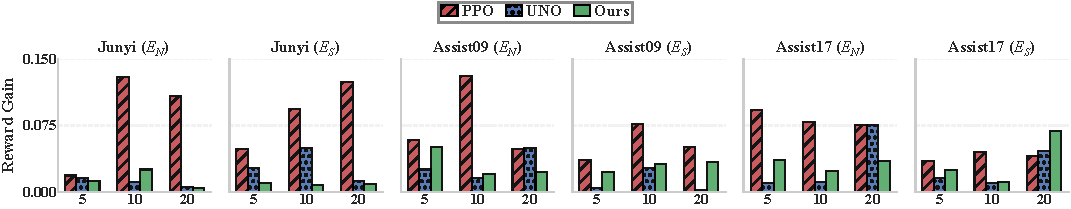
\includegraphics[width=0.98\textwidth]{p1_p12_diff_comparison.pdf} % 插入图片并设置宽度
    \caption{Reward transfer study. The vertical axis denotes the average performance gain, computed as $\text{Hybrid Process Reward}-\text{Discrete-Attainment Reward}$.}
    \label{fig:diff-comparison} % 用于交叉引用的标签
\end{figure*}
\subsection{Stability Analysis}

为验证整体框架在更换知识点规划算法后的稳定性，我们固定监督式局部习题执行器不变，仅将 L-Agent 分别替换为 AC、DQN\cite{mnih2015human}、SAC\cite{haarnoja2018soft} 和本文采用的 PPO 版本，并统计不同步数下的平均学习收益。表~\ref{tab:stability_analysis} 表明，使用 PPO 的本文方案在两个数据集上的 $E_N$ 和 $E_S$ 指标上整体最优；同时，无论采用哪种知识点策略，学习收益都能随步数增加而逐步提升，说明在更换 L-Agent 后，整体规划--执行框架仍能保持较稳定的优化趋势。进一步地，可以看到 DQN 在大多数设置下都落后于 AC、SAC 和 PPO，说明仅依赖价值估计的离散动作策略在当前知识点规划任务上相对较弱，而 actor-critic 类方法能够更好地适应该类序列决策过程。该结果从侧面说明，本文方法不仅在算法选择上具有优势，也具有较好的结构稳定性。

\begin{figure}[t] % 位置参数，见下文解释
    \centering % 图片居中
    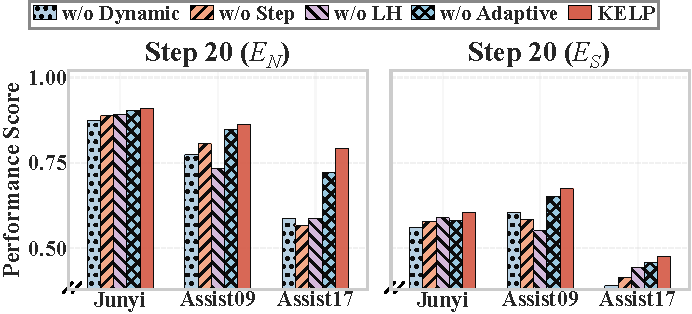
\includegraphics[width=\columnwidth]{ablation_study_step20.pdf} % 插入图片并设置宽度
    \caption{Ablation study of each optimization module}
    \label{fig:Ablation study} % 用于交叉引用的标签
\end{figure}
\subsection{Local Executor Effectiveness Analysis}
为进一步验证局部习题执行器评分机制的有效性，我们在测试阶段分别执行排序第 1 至第 5 的候选习题，并比较不同选择下的最终表现，如图~\ref{fig:effctiveness Analysis} 所示。其中，等级 1 表示当前状态下由执行器判定为$\hat{r}_{t}$分数最高的习题，等级越大表示所选习题在候选集合
中的匹配分数越低。从结果来看，三个数据集整体上都呈现出一致趋势：随着所选习题的等级从 1 下降到 5，$E_N$ 与 $E_S$ 均整体下降，说明执行器给出的分数能够较好反映习题对当前知识点目标的真实适配性。其中，Junyi 与 Assist17 上的下降更为明显，尤其在步数较大时，高排名习题与低排名习题之间的差距进一步拉大；相比之下，Assist09 上不同排序之间的差距相对更平缓，但最优结果仍出现在排序最靠前的位置。总体而言，该实验说明局部习题执行器的评分不仅能够用于候选重排，而且与真实学习收益具有较强一致性，从实验上支持了监督式局部习题执行设计的合理性。
\begin{figure}[t] % 位置参数，见下文解释
    \centering % 图片居中
    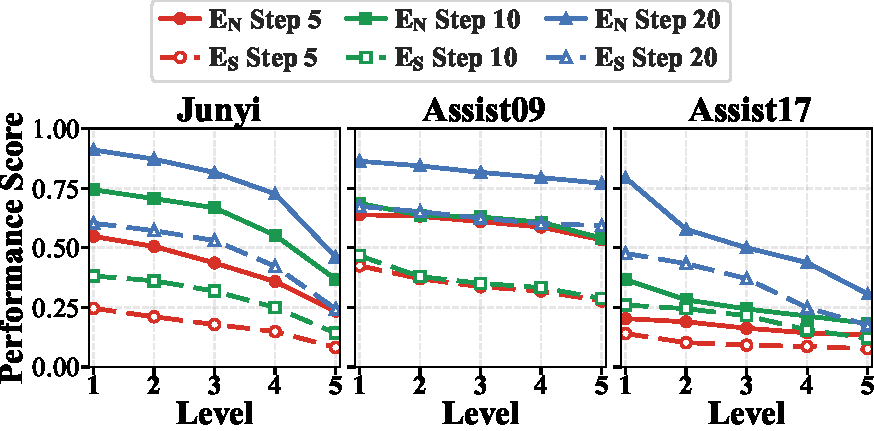
\includegraphics[width=\columnwidth]{adaptability_experiment_font_large.pdf} % 插入图片并设置宽度
    \caption{Performance comparison of exercises at different local executor score levels.}
    \label{fig:effctiveness Analysis} % 用于交叉引用的标签 
\end{figure}

\subsection{Case Study}
为进一步分析不同方法的推荐行为，我们展示一个学习路径案例，如图~\ref{fig:case_study} 所示。可以看到,$E_N$指标并不能在每一步都发生变化,当只使用离散达成收益作为过程奖励时不可避免地出现零奖励,从而影响对于这一步动作有效性的判断,这显示地证明了引入连续掌握收益构建细粒度奖励机制的重要性.我们的方法最快将学习目标推进到合格水平，表现出更高的目标达成效率。进一步地，图中的 (a)、(b) 和 (c) 都属于基于步级过程奖励构建的方法，因此在学习过程中整体收益保持逐步上升，没有出现明显的中途退化；相比之下，使用终局奖励的 SRC 在初始阶段出现了学习收益下降，这种现象在真实学习场景中可能打击学生的学习积极性，并削弱其对推荐系统的信任。另一个值得注意的现象是，UNO 在该案例中多次重复推荐同一知识点，这与数据中存在连续重复学习同一知识点的模式有关；由于 UNO 属于序列式推荐方法，更容易捕捉并放大此类模式。因此，推荐系统除关注收益提升外，还需要合理控制知识点重复学习的频率。
\begin{figure}[t]
\centering
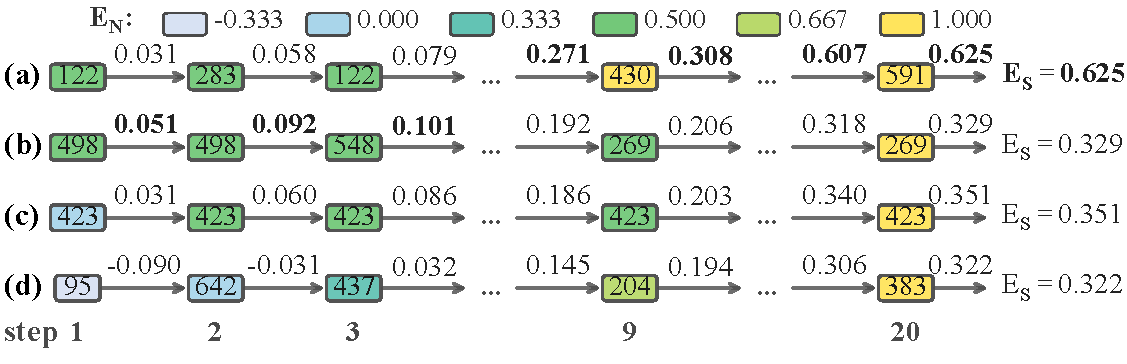
\includegraphics[width=\columnwidth]{case_study.pdf}
\captionsetup{labelfont=bf,textfont=bf}
\caption{Curriculum path case study. (a), (b), (c), and (d) denote KELP, PPO, UNO, and SRC, respectively.}
\label{fig:case_study}
\end{figure}
\section{Conclusion}
本文针对目标导向学习路径推荐中细粒度状态变化、规划反馈与预算感知不足的问题，提出分层两阶段细粒度学习路径推荐框架 KELP。该框架通过统一状态估计连接强化学习知识点规划器与监督式局部习题执行器，并采用“一步一知识点一习题”的决策粒度，结合双阶段知识点规划、连续掌握收益与状态感知的局部选题，实现知识点规划和习题反馈的协同决策。

在 Junyi、Assist09 和 Assist17 上的实验表明，KELP 在多数设置下取得了更优的学习收益；消融与扩展实验进一步验证了关键模块的有效性、连续掌握收益的可迁移性，以及习题匹配分数与真实学习收益的一致性。未来将结合真实在线交互数据验证框架的实际适用性，并探索更复杂的学习目标与长期学习场景。
\printbibliogCEraphy
\end{document}